%  !TeX  root  =  user_guide.tex 

\section{Georeferencer Plugin}

% when the revision of a section has been finalized, 
% comment out the following line:
%\updatedisclaimer

The Georeferencer Plugin is a tool for generating world files for rasters.
It allows you to reference rasters to geographic or projected coordinate 
systems by creating a new GeoTiff or by adding a world file to the 
existing image. The basic approach to georeferencing a raster is to locate 
points on the raster for which you can accurately determine their coordinates. 

\minisec{Features}

\begin{table}[h]\index{Georeferencer!tools}
\begin{tabular}{|m{1cm}|m{6cm}|m{1cm}|m{6cm}|}
 \hline \textbf{Icon} & \textbf{Purpose} & \textbf{Icon} &
 \textbf{Purpose} \\
 \hline 
\includegraphics[width=0.7cm]{mActionAddRasterLayer} & Open raster &
 
\includegraphics[width=0.7cm]{mActionStartGeoref} & Start georeferencing \\
 \hline 
\includegraphics[width=0.7cm]{mActionGDALScript} & Generate GDAL script &
 
\includegraphics[width=0.7cm]{mActionFileOpen} & Load GCP Points \\
 \hline 
\includegraphics[width=0.7cm]{mActionFileSave} & Save GCP Points as &
 
\includegraphics[width=0.7cm]{mActionOptions} & Transformation settings \\
 \hline 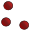
\includegraphics[width=0.7cm]{mActionCapturePoint} & Add Point &
 
\includegraphics[width=0.7cm]{mActionDeleteSelected} & Delete Point \\
 \hline 
\includegraphics[width=0.7cm]{mActionMoveFeature} & Move GCP Point &
 
\includegraphics[width=0.7cm]{mActionPan} & Pan \\
 \hline 
\includegraphics[width=0.7cm]{mActionZoomIn} & Zoom in &
 
\includegraphics[width=0.7cm]{mActionZoomOut} & Zoom out \\
 \hline 
\includegraphics[width=0.7cm]{mActionZoomToLayer} & Zoom to layer &
 
\includegraphics[width=0.7cm]{mActionZoomLast} & Zoom Last \\
 \hline 
\includegraphics[width=0.7cm]{mActionZoomNext} & Zoom Next &
 
\includegraphics[width=0.7cm]{mActionLinkGeorefToQGis} & Link Georeferencer to QGIS \\
 \hline 
\includegraphics[width=0.7cm]{mActionLinkQGisToGeoref} & Link QGIS to Georeferencer &
 &  \\
\hline
\end{tabular}
\caption{Georeferencer Tools}\label{tab:georeferencer_tools}
\end{table}

\minisec{Usual procedure}

As X and Y coordinates (DMS (dd mm ss.ss), DD (dd.dd) or projected coordinates 
(mmmm.mm) which correspond with the selected point on the image, two 
alternative procedures can be used: 

\begin{enumerate}
\item The raster itself sometimes provides crosses with coordinates 
`written' on the image. In this case you can enter the coordinates manually.
\item Using already georeferenced layers, this can be either vector or 
raster data that contain the same objects/features that you have on 
the image that you want to georeference and the projection you want to 
have your image. In this case you can enter the coordinates by 
clicking on the reference dataset loaded in QGIS map canvas.
\end{enumerate}

The usual procedure for georeferencing an image involves selecting multiple 
points on the raster, specifying their coordinates, and choosing a relevant 
transformation type. Based on the input parameters and data, the plugin will 
compute the world file parameters. The more coordinates you provide, the 
better the result will be.

The first step is to start QGIS, load the Georeferencer Plugin (see Section 
\ref{sec:load_core_plugin}) and click on the 
\toolbtntwo{georeferencer}{Georeferencer} icon which appears in the 
QGIS toolbar menu. The Georeferencer Plugin dialog appears as shown 
in Figure \ref{fig:georefplugin}.
  
For this example, we are using a topo sheet of South Dakota from SDGS. 
It can later be visualized together with the data from the GRASS spearfish60 
location. You can download the topo sheet here: 
\url{http://grass.osgeo.org/sampledata/spearfish\_toposheet.tar.gz}

\begin{figure}[ht]
\centering
  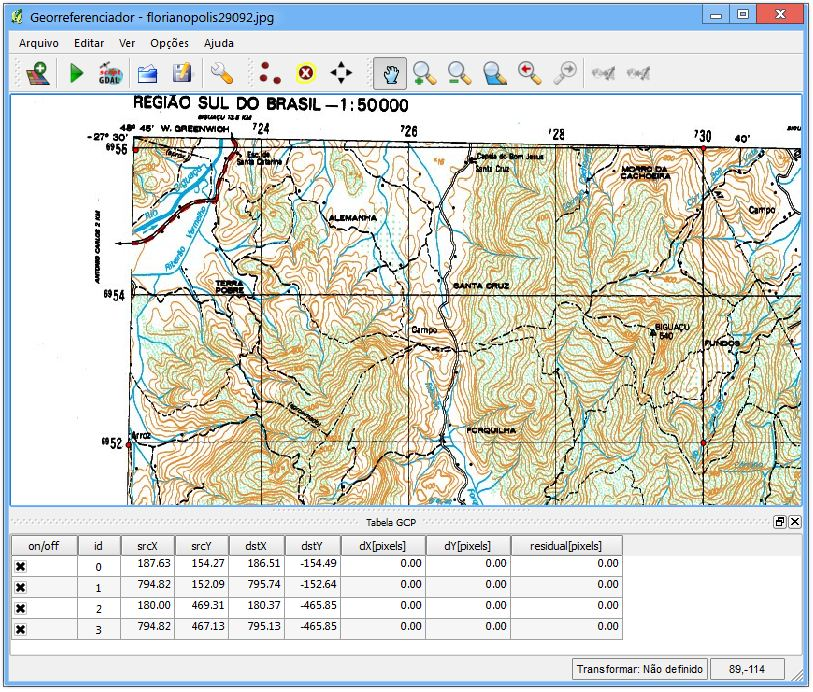
\includegraphics[clip=true, width=12cm]{georefplugin}
  \caption{Georeferencer Plugin Dialog \nixcaption}\label{fig:georefplugin}
\end{figure}

\minisec{Entering ground control points (GCPs)}\label{georeferencer_entering}

\begin{enumerate}
\item To start georeferencing an unreferenced raster, we must load it using 
the 
\includegraphics[width=0.7cm]{mActionAddRasterLayer} button. The raster 
will show up in the main working area of the dialog. Once the raster is 
loaded, we can start to enter reference points.
\item Using the \toolbtntwo{mActionCapturePoint}{Add Point} button, add 
points to the main working area and enter their coordinates 
(See Figure \ref{fig:choose_points}). For this procedure you have two 
options:

\begin{enumerate}
\item Click on a point in the raster image and enter the X and Y coordinates manually
\item Click on a point in the raster image and choose the button 
\toolbtntwo{pencil}{from map canvas} to add the X and Y coordinates with the help 
of a georeferenced map already loaded in the QGIS map canvas.
\item With the 
\includegraphics[width=0.7cm]{mActionMoveFeature} button, you can move 
the GCPs in both windows, if they are at the wrong place. 
\end{enumerate}
\item Continue entering points. You should have at least 4 points, and the 
more coordinates you can provide, the better the result will be. There are 
additional tools on the plugin dialog to zoom and pan the working area in 
order to locate a relevant set of GCP points.
\end{enumerate}

\begin{figure}[ht]
\centering
  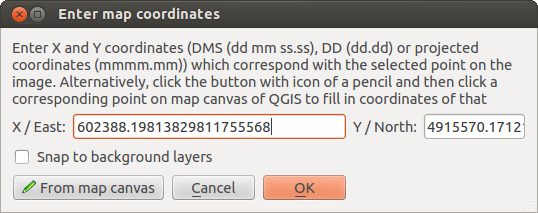
\includegraphics[clip=true,width=5cm]{choose_points}
  \caption{Add points to the raster image \nixcaption}\label{fig:choose_points}
\end{figure}

The points that are added to the map will be stored in a separate text 
file ([filename].points) usually together with the raster image. 
This allows us to reopen the Georeferencer plugin at a later date and add 
new points or delete existing ones to optimize the result. The points file 
contains values of the form: mapX, mapY, pixelX, pixelY. You can use the 

\includegraphics[width=0.7cm]{mActionFileOpen} 'Load GCP Points' and 

\includegraphics[width=0.7cm]{mActionFileSave} 'Save GCP Points' buttons to 
manage the files. Within the GCP table you can click on a column header and 
therewith enable e.g. numerical sorting. The GCP list is automatically updated.

\minisec{Defining the transformation settings}\label{georeferencer_transformation}

After you have added your GCPs to the raster image, you need to define the 
transformation settings for the georeferencing process. 

\begin{figure}[ht]
\centering
  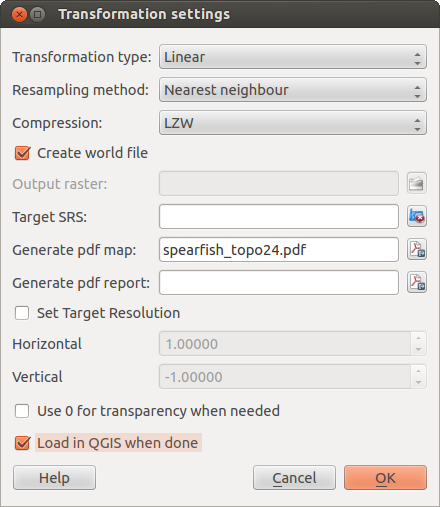
\includegraphics[clip=true,width=5cm]{transformation_settings}
  \caption{Defining the georeferencer transformation settings \nixcaption}\label{fig:georef_transform}
\end{figure}

\minisec{Available Transformation algorithms}

Depending on how many ground control point you have captured, you may want 
to use different transformation algorithms. Choice of transformation 
algorithm is also dependent on the type and quality of input data and 
the amount of geometric distortion that you are willing to introduce 
to final result.

Currently, following algorithms are available: 

\begin{itemize}[label=--]
\item The \textbf{Linear algorithm} is used to create a world-file, and is different 
from the other algorithms, as it does not actually transform the raster. 
This algorithm likely won't be sufficient if you are dealing with scanned 
material.
\item The \textbf{Helmert transformation} performs simple scaling and rotation 
transformations. 
\item The \textbf{Polynomial algorithms} 1-3 are among the most widely 
used algorithms 
for georeferencing, and each one differs by the degree of distortion 
introduced to match source and destination ground control points. The 
most widely used polynomial algorithm is the second order polynomial 
transformation, which allows some curvature. First order polynomial 
transformation (affine) preserves colliniarity and allows scaling, 
translation and rotation only.
\item The \textbf{Thin plate spline (TPS) algorithm} is a more 
modern georeferencing  method, which is able to introduce local 
deformations in the data. This algorithm is useful when very low 
quality originals are being georeferenced.
\end{itemize}

\minisec{Define the Resampling method}

The type of resampling you choose will likely depending on your input data
and the ultimate objective of the exercise. If you don't want to change
statistics of the image, you might want to choose Nearest neighbour,
whereas a Cubic resampling will likely provide a more smoothed result.

It is prossible to choose between five different resampling methods.

\begin{enumerate}
\item Nearest neighbour
\item Linear
\item Cubic
\item Cubic Spline
\item Lanczos
\end{enumerate}

\minisec{Define the transformation settings}

There are several options that need to be defined for the georeferenced output 
raster. 

\begin{itemize}[label=--]
\item The checkbox \checkbox{Create world file} is only available, if 
you decide to use the linear transformation type, because this means that 
the raster image actually won't be transformed. In this case, the field 
Output raster is not activated, because only a new world-file will be 
created.
\item For all other transformation type you have to define an \textbf{Output 
raster}. As default a new file ([filename]\_modified) will be created in 
the same folder together with the original raster image.   
\item As a next step you have to define the \textbf{Target SRS} 
(Spatial Reference System) for the georeferenced raster 
(see section \ref{label_projections}). 
\item If you like, you can \textbf{generate a pdf map} and also \textbf{a 
pdf report}. The report ncludes information about the used transformation 
parameters. An image of the residuals and a list with all GCPs and their 
RMS errors.
\item Furthermore you can activate the \checkbox{Set Target Resolution} 
checkbox and define pixel resolution of the output raster. Default horizontal 
and vertical resolution is 1,      
\item The \checkbox{Use 0 for transparency when needed} can be activated, if 
pixels with the value 0 shall be visualized transparent. In our example 
toposheet all white areas would be transparent.
\item Finally \checkbox{Load in QGIS when done} loads the output raster 
automatically into the QGIS map canvas when the transformation is done.
\end{itemize}

\minisec{Show and adapt raster properties}

Clicking on the \dialog{Raster properties} dialog in the \dropmenuopt{Settings} menu 
opens the raster properties of the layer that you want to georeference.   

\minisec{Configure the georeferencer}

\begin{itemize}[label=--]
\item You can define if you want to show GCP coordiniates and/or IDs.
\item As residual units pixels and map units can be chosen.
\item For the PDF report a left and right margin can be defined and you can 
also set the paper size for the PDF map.
\item Finally you can activate to \checkbox{show georeferencer window docked}. 
\end{itemize}

\minisec{Running the transformation}\label{georeferencer_running}

After all GCPs have been collected and all transformation settings are 
defined, just press the button 
\includegraphics[width=0.7cm]{mActionStartGeoref} 
'Start georeferencing' to create the new georeferenced raster.


